\documentclass[a4paper,english, 11pt]{article}

\usepackage{siunitx} 
\usepackage[hidelinks]{hyperref}
\usepackage[a4paper,inner=2.5cm,outer=2.5cm,top=2.5cm,bottom=2.5cm,pdftex]{geometry} 
\usepackage{array}
\usepackage{fancyhdr}
\usepackage{graphicx}     
\usepackage{natbib}
\usepackage{hyperref}
\usepackage{tcolorbox}
\usepackage{titling}
\usepackage{listings}
\usepackage{color}
\usepackage{textcomp}

\newcommand{\subtitle}[1]{%
  \posttitle{%
    \par\end{center}
    \begin{center}\large#1\end{center}
    \vskip0.5em}%
}
\newcommand{\emailme}{\href{mailto:data.nleg@unis.no}{data.nleg@unis.no}}

\definecolor{dkgreen}{rgb}{0,0.6,0}
\definecolor{gray}{rgb}{0.5,0.5,0.5}
\definecolor{mauve}{rgb}{0.58,0,0.82}

\graphicspath{{../Images/}} 
\bibliographystyle{agsm}

\title{How to publish FAIR Nansen Legacy datasets}
\subtitle{A complete step by step guide}
\date{\today\\v1.0}
\author{Luke Marsden (\emailme)}

\begin{document}
\maketitle
\tableofcontents
\pagestyle{fancy}
\newpage
\section{Introduction}
\label{s:Introduction}

Publishing your data benefits both you and the broader scientific community. It supports transparency and reproducibility of your research, and allows others to work with your data, thus promoting collaboration. Published datasets are visible and citeable, and look great on your job and grant applications. As outlined in both the data management plan \citep{aendmp2021} and data policy \citep{aendatapolicy2021} we are committed to publishing FAIR data \citep{wilkinson2016fair}, meaning that data should be:

\begin{itemize}
\item Findable: Data and metadata are findable by humans and computers and assigned a persistent identifier (e.g. DOI).
\item Accessible: Data and metadata can be freely and openly accessed, allowing authentication and authorization if necessary.
\item Interoperable: Data and metadata use standardised terms (common vocabularies) and file structures allowing use in different applications or workflows with minimal manual intervention. 
\item Reusable: Data and metadata are richly and clearly described for humans and computers to understand and have a clear data usage license. 
\end{itemize}

When you publish an paper in a scientific journal, it is now often a requirement that the data are published in a data repository, usually making the data findable and accessible. However, this does not necessarily mean that the data are easy for someone else to use. Here, we will go step-by-step through how to publish FAIR datasets in the Nansen Legacy project.

\section{Selecting a suitable file type and conventions}
\label{s:FileType}

The first step is to identify what type of data you are working with. This will determine what file format you should convert your data to, and which conventions should be used for the metadata. For most Nansen Legacy datasets, NetCDF-CF (Network Common Data Form - Climate and Forecast) or Darwin Core Archive (DwCA) should be used. See Table \ref{t:netcdf_vs_dwca} for examples. Please email \emailme \ if you are unsure or if you think your data are an exception. NetCDF-CF and DwCA are self-describing file types, meaning that they include rich metadata that enables the data user to understand and use the data unaided.

\begin{table}[h!]
  \begin{center}
    \label{t:netcdf_vs_dwca}
    \begin{tabular}{l|r} % <-- Alignments: 1st column left, 2nd middle and 3rd right, with vertical lines in between
      \textbf{NetCDF-CF} & \textbf{DwCA}\\
      \hline
      Physical data & Biodiversity data\\
      Physical oceanography data & Ecological data\\
      Atmospheric data & Measurements of species/individual\\
      Sea water temperature & Primary production rate\\
      Particulate organic carbon in sea water & Age of fossil\\
      Wind speed & Fatty acids in fish\\
      Sea ice thickness & List of species from processed DNA data\\
      Chlorophyll A concentration & Virus diversity\\
      
    \end{tabular}
    \caption{Examples of data that should be stored as either NetCDF-CF or DwCA}
  \end{center}
\end{table}

%You can refer to XXXX, a spreadsheet that lists various parameters measured in the Nansen Legacy project, and the file type, standard name and units that should be used when publishing the data. If the parameter that you are working with is missing from this spreadsheet, please contact \emailme \ so it can be added.

If your data should be converted to NetCDF-CF, go to section \ref{s:NetCDF-CF}.

If your data should be converted to DwCA, go to section \ref{s:DwCA}.

\newpage
\section{NetCDF-CF}
\label{s:NetCDF-CF}

Some information first about NetCDF-CF. 

NetCDF (Network Common Data Forum) is a file format that is used for storing multidimensional scientific data in grids. There are several components of a NetCDF file. Scientific data (such as wind speed, sea water temperature etc.) are stored as \textit{variables}, whose values are stored in an array or multidimensional grid. \textit{Dimensions} may be for example time or a spatial coordinate.

When creating a NetCDF file, one must first define the dimensions. A multidimensional grid can be defined by using more than one dimension, e.g. longitude, latitude and time (Figure \ref{fig:netcdf}). The file creator then defines which dimensions each variable uses - this may be one, multiple or all of the defined dimensions. For the example in Figure \ref{fig:netcdf}, we have values for the wind speed variable at different latitudes, longitudes and times. However, if we wanted to include a second variable to be assumed constant through time, we could only assign latitude and longitude to that variable. We also define \textit{coordinate variables} that correspond to each of the dimensions. In Figure \ref{fig:netcdf}, we have a \textit{longitude} dimension with a length of 3. The corresponding \textit{longitude} variable defines what the actual values are at each point in the grid. 

Values must be assigned for the variable at every point in the multidimensional grid. There may be some points in the grid where a value does not exist. In these cases, a \textit{fill value} is defined. This fill value is a constant value that is unrealistic, e.g. orders of magnitude too high, or a negative value.

\begin{figure}[htb]
    \tcbox[colback=white]{
    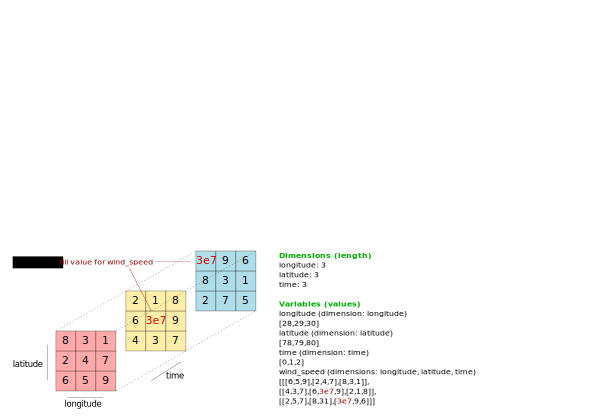
\includegraphics[width=0.93\textwidth]{netcdf.png}
    }
    \caption{\label{fig:netcdf}
        Visualisation of a multidimensional netCDF file, with 3 dimensions: longitude, latitude and time.
        Each dimension has a set length (each 3 in this case), and the values
        for the dimension are stored as a \textit{coordinate variable} with the same name.
        Each variable has values defined, and references dimensions which define the location of each value in the grid. The wind$\_$speed variable has 3 dimensions in this case (longitude, latitude and time). Values for the wind$\_$speed variable are plotted, and a fill value of 3e7 has been used where no measurement was taken. 
    }
\end{figure}

A NetCDF file also includes \textit{variable attributes} (metadata that describe each variable) and \textit{global attributes} (metadata that describe the file as a whole). Commonly accepted conventions should be used that define what metadata should be included,  what names should be used for each metadata term, and descriptions that describe each term and how to populate it. Conventions ensure consistency between data created by different users, and make the data both human and machine readable, required for the data to be interoperable and reusable (FAIR - section \ref{s:Introduction}). We also reference what conventions we have used as a global attribute (term: \href{https://www.unidata.ucar.edu/software/netcdf/conventions.html}{Conventions}). 

The Climate and Forecast (CF) conventions (hence NetCDF-CF) are \textit{use} metadata, that instruct someone on how to use the data. They define \textit{standard names} and units to be used for different variables, with descriptions. The official documentation for the NetCDF-CF conventions can be found here (\url{http://cfconventions.org/}).

We also use the Attribute Convention for Data and Discovery (ACDD), which are \textit{discovery} metadata that help someone to find the data. They define variable and global attributes that are recommended for use. We will outline which attributes to use for Nansen Legacy datasets in sections \ref{ss:globalattributes} (global attributes) and \ref{ss:variableattributes} (variable attributes). Information on ACDD can be found at \url{https://wiki.esipfed.org/Attribute_Convention_for_Data_Discovery}. 

\subsection{How to structure your data collection}
\label{ss:structurecollection}

What dimensions do your data have? A single depth profile? Multiple depth profiles? A time series? A grid of latitude and longitudes an discrete time intervals? Or something more complicated?

This will dictate how to structure your data collection. There are different approaches, but we advise that each NetCDF-CF file should be as simple as possible. This might mean dividing your data into multiple small files, that can be stored in a single data collection. For example, one file for each depth profile. This approach has several advantages:

\begin{itemize}
\item Each file is easier to create.
\item Each file can be specifically described with its own set of metadata.
\item Each file is easier to understand.
\item If someone is interested in only a subset of the data, they can easily access these without having to download and open the rest of the data too.
\item Each file gets its own DOI. You can also get a DOI for the full data collection for those who want to cite everything.
\item Imagine you have multiple depth profiles. To store them all in the same file, you would have to have a longitude and latitude dimension. If using separate files, each file can state the longitude and latitude in the metadata, and only one dimension (depth) is required.
\end{itemize}   

Consider how many files you will need to create. Consider what is constant for each file (global attributes), what varies within each file (variables and dimensions) and what varies between the different files.

If each data point corresponds to a single event in the metadata catalogue (i.e. a single row in the sample logs) the event ID can also be stored in this file, to link the metadata catalogue and data together. We will get back to how to do this later (section \ref{ss:convertingnetcdf}).

\subsection{Dimensions and variables: cleaning up your input data}
\label{ss:dimensionsvariables}

You should now know what your dimensions and variables will be for each file. These might correspond to individual columns in a spreadsheet or CSV file for example, or perhaps a subset of a column. You can now focus on preparing these data to make converting them to NetCDF easier.

These tips are advised, not mandatory. You can alternatively implement most of these steps within the script your write to convert your data to netCDF-CF. 

\begin{enumerate}
\item Do you have all the columns you need?
\begin{itemize}
\item Collect all the columns you need in one file.
\item If metadata associated with your data was logged in \href{https://sios-svalbard.org/cgi-bin/darwinsheet/?setup=aen}{Nansen Legacy sample logs}, you should have corresponding Event IDs (one per data point or one per data collection in some cases). The metadata you logged are updated before they are uploaded to the \href{https://sios-svalbard.org/aen/tools}{metadata catalogue on SIOS} - cleaned and errors corrected. 
Please contact me to retrieve this updated metadata and provide me with a list of event IDs.
%You can retrieve the updated metadata at REF. You will publish some of these metadata with your data. This tool also outputs event dates (including times) in \href{https://en.wikipedia.org/wiki/ISO_8601}{ISO 8601} format, necessary for publishing.    
\end{itemize}
\item For the data columns (not metadata), check whether standard names exist for each variable that you will publish.
\begin{itemize}
\item Variables:
Select a standard name for each variable from \href{https://cfconventions.org/standard-names.html}{https://cfconventions.org/standard-names.html}. Use this as your column header. Pay attention to the description and units. It may be necessary to convert your data to the units listed. If no suitable standard name exists, please email \emailme .
\item Dimensions: \textit{time}, \textit{latitude}, \textit{longitude} and \textit{depth} are all accepted standard names for dimensions and their respective \textit{coordinate variables}.
\end{itemize}
\item Clean each column that will be used. The key here is to be consistent:
\begin{itemize}
\item Don't include text in columns that should contain only numbers.
\item Make sure all values make sense (e.g. no negative volumes).
\item If no real value was measured, leave it blank or assign a fill value. This fill value should be an unrealistic value, e.g. excessively high, or negative. Use the same fill value/blank for each case in the column. Different values can be used for different variables. Make a note of this fill value - it will be provided as a variable attribute later, which we will cover in section \ref{ss:convertingnetcdf}. 
\end{itemize}
\end{enumerate}

\subsection{Global attributes}
\label{ss:globalattributes}

Global attributes provide discovery metadata that are related to each NetCDF-CF files as a whole. Each attribute name is taken from a controlled vocabulary (section \ref{ss:controlledvocabularies}). This means that it has a description associated with it that is findable online. This should instruct you how to fill in each term, and help someone working with your data to understand the contents.

A list of which global attributes can be included (required and recommended) can be found here:
\href{https://adc.met.no/node/4}{https://adc.met.no/node/4}

Here is some extra help for some of the attributes, specific to Nansen Legacy, which can be seen as additional to the help linked above (not in place of):
\begin{itemize}
\item \textbf{id}: If a single event ID in the metadata catalogue is related to the whole file, and only that file, it can be included here. 
%Otherwise, a different UUID must be generated. This UUID should be reproducible, in case you want to update the file. Version 5 UUIDs are generated by `hashing a namespace identifier'. This means that they are created from text, and the text can be recovered from the UUID also.
\item \textbf{keywords}: The keyword should be taken from the GCMD (Global Change Master Directory) keywords, and should be written like:

EARTH SCIENCE $>$ ATMOSPHERE $>$ ATMOSPHERIC WINDS $>$ SURFACE WINDS $>$  WIND SPEED

They can be selected from \url{https://gcmd.earthdata.nasa.gov/static/kms/}.
If multiple keywords are required, please separate using semicolons ;

EARTH SCIENCE $>$ ATMOSPHERE $>$ ATMOSPHERIC WINDS $>$ SURFACE WINDS $>$  WIND SPEED; EARTH SCIENCE $>$ ATMOSPHERE $>$ ATMOSPHERIC WINDS $>$ SURFACE WINDS $>$  WIND DIRECTION

\item \textbf{keywords\_vocabulary}: simply write `GCMD'
\item \textbf{creator}: This is the contact person for the data, who is principally responsible for the data, and who will be listed as authors if the data are cited. Can be multiple people separated by commas. creator\_institution, creator\_email, creator\_url should be provided for every creator, again comma-separated, even if they are from the same institution. It is otherwise ambiguous whether for example a single creator\_institution refers to all the creators or just the first.  
\item \textbf{publisher}: Provide details for the data centre where you are publishing your data. See section \ref{s:datacentre}.
\item \textbf{license}: According to the project data policy \citep{aendatapolicy2021}, all data should be published with the Creative Common Attribution license (\url{https://creativecommons.org/licenses/by/4.0/}). Include this URL for the attribute value. 
\item \textbf{acknowledgements}: Refer to the Research Council of Norway who fund the project (The Nansen Legacy (RCN 276730), and anyone you want to acknowledge involved in recording, analysing or processing the data up to this point for example.
\end{itemize}

Additional global attributes can also be included, defined by the user. Try to use attribute names that will be understandable to someone outside of the project, but they don't have to be standardised. In the Nansen Legacy project, we recommend also including the following global attributes are included as a minimum. 

\begin{itemize}
\item {sampling$\_$protocols}: Cite the published Nansen Legacy sampling protocols. Remember to refer to a specific version and section within. You may refer to other published work that outlines the methods if not included in the sampling protocols.
\item {sea$\_$floor$\_$depth$\_$below$\_$sea$\_$surface}: Can be taken from the 'Bottom depth in meters' column in the metadata catalogue.
\item {metadata$\_$link}: DOI provided for the file by the data repository.
\end{itemize}   

Make sure you have all of this information before you proceed to section \ref{ss:convertingnetcdf}.

\subsection{Variable attributes}
\label{ss:variableattributes}

Variable attributes provide metadata that describe each variable. A list of variable attributes can be found at \url{https://wiki.esipfed.org/Attribute_Convention_for_Data_Discovery_1-3}, and we recommend that all the \textit{highly recommended variable attributes} are used.

Notes:
\begin{itemize}
\item The standard$\_$name is taken from the CF conventions (\url{https://cfconventions.org/standard-names.html}). 
\item You should convert your variable to the units stated by the standard$\_$name in the CF conventions.
\item If a suitable standard$\_$name does not exist, please contact \emailme . By liaising with the standards body, a new standard$\_$name can be proposed and added. Expanding existing standards benefits the broader scientific community.
\item The long$\_$name is your description of what the variable represents.  
\end{itemize}

For coordinate variables, use the following variable attributes, and make sure your data are structured accordingly.

\begin{center}
\begin{tabular}{ |c|p{0.28\textwidth}|p{0.38\textwidth}|p{0.08\textwidth}| } 
\hline
standard\_name & long\_name & units & positive \\
\hline
time & time & days since 2018-01-01 & \\
& & seconds since 2020-07-10T12:00:00Z & \\ 
latitude & decimal latitude in degrees north & degrees\_north & \\
longitude & decimal longitude in degrees east & degrees\_east & \\
depth & depth below sea level & m & down \\
\hline
\end{tabular}
\end{center}

Make sure you have all of this information before you proceed to section \ref{ss:convertingnetcdf}.

\newpage
\subsection{Converting to NetCDF-CF}
\label{ss:convertingnetcdf}

Your input data should now be ready to convert to NetCDF-CF. There are different ways to do this, depending on your data and your experience.

\begin{itemize}
\item Rosetta (\url{http://tomcat.nersc.no/rosetta/})
\begin{itemize}
\item Creating NetCDF-CF files with a simple graphical user interface. 
\item Does not require any coding experience.
\item Suitable for tabular data (from Excel to NetCDF-CF for example).
\item Not suitable for creating complicated data files with lots of dimensions.
\item Inefficient if you plan to create a large number of similar files, as each will have to be created individually - though templates can be used to speed this up. Slow compared to creating similar files collectively in a script with a `for loop' for example. 
\item To proceed with this option, go to section \ref{ss:Rosetta}.
\end{itemize}
\item Writing a script
\begin{itemize}
\item Can write a single script to create all your files (time efficient). 
\item Reusable with small tweaks for similar files in the future.
\item More control (not restricted by what Rosetta allows).
\item Learning curve if you don't code often.
\item Python (netCDF4 or xarray libraries) - xarray introduced in section \ref{ss:xarray}
\item R - introduced in section \ref{ss:R}
\item MATLAB, Fortran...   
\end{itemize}
\end{itemize}

\subsubsection{Rosetta (for those who don't like to code)}
\label{ss:Rosetta}

For people who don't like to code, Rosetta provides a graphical user interface with which you can create NetCDF-CF files.

\url{http://tomcat.nersc.no/rosetta/}

One disadvantage is that this approach takes a long time if you have lots of similar files. Also, it can be more difficult to create complex multidimensional files. However, for simple files, this is an effective method that is easy to learn.

A user manual can be found here:\\
\url{https://drive.google.com/file/d/1Ss7G2kHZipBWLn28CdZooxDiXLztRQlp/view}.

I will now go step-by-step through an example specific to Nansen Legacy. Let's consider an example where we have a depth profile at a single station. We will use a dummy dataset that you can find here:
\url{https://github.com/SIOS-Svalbard/AeN_doc/blob/master/NetCDF-CF_example_scripts_and_data/chlorophyll_a_depth_profiles.xlsx}

\begin{enumerate}
\item XLSX files are not currently supported. Convert your file to CSV, ASCII, or XLS. You will also need to divide your data into 1 file per station.
\item Go to \url{http://tomcat.nersc.no/rosetta/}.
\item Select \textit{Convert a file to the netCDF format and create a new template}.
\item Select \textit{Single CTD/XBT cast (profile)} and hit \textit{Next}.
\item Upload the file and hit \textit{Next}.
\item Select your header row and hit \textit{Next}.
\item Specify the delimiter and hit \textit{Next}. You will be able to check that the data have been divided into columns correctly on the next page.
\item Select which columns should be stored as variables in the NetCDF file. Both coordinate variables and data variables should be selected. In this case:
\begin{itemize}
\item eventID:
\begin{enumerate}
\item Use \textit{eventID} as the \textit{variable name}.
\item This is not a coordinate variable.
\item The data type is \textit{text}. 
\item For \textit{Instrument Description} enter \textit{NA}.
\item For \textit{Missing Value} enter \textit{None}.
\item For \textit{Variable Description} enter:\\
\textit{The event ID is a universally unique ID assigned to each sample. Additional metadata related to each sample can be found be visiting the Nansen Legacy hierachical metadata catalogue hosted on the SIOS webpage and searching for for the eventID in the Fulltext search.}.
\item Hit \textit{done}.
\end{enumerate}
\item sampleDepthInMeters:
\begin{enumerate}
\item The \textit{variable name} should be depth.
\item It is a coordinate variable.
\item Select \textit{altitude} as the type of coordinate variable.
\item The data are integers
\item Fill in the required metadata and any recommended or additional metadata you wish to add. 
\end{enumerate}
\item mass\_concentration\_of\_chlorophyll\_a\_in\_sea\_water:
\begin{enumerate}
\item Assign a variable name selected from \url{http://cfconventions.org/standard-names.html}. As you begin to type the variable, you will be able to select it from a drop-down list that will appear.
\item This is not a coordinate variable.
\item These data are decimal, so select \textit{float}.
\item Fill in the required metadata and any recommended or additional metadata you wish to add. 
\begin{itemize}
\item \textit{variable description} should be in your own words. Try to be thorough and describe any processing that has been applied to create the data. 
\item \textit{units} should be the units provided for the standard name where possible. This may involve converting your data.
\end{itemize}
\end{enumerate}
\item The remaining columns contain values that are constant for all samples in the file. These are global attributes, and we will define these later. For now, select each of the remaining columns in turn and select \textit{Do not use this column of data}.
\end{itemize}
\item Enter the site specific information. Pay attention to the ? symbols for instructions on how to format each field. In our case, since we have used the TOOL tool to retrieve metadata from the metadata catalogue, we can just copy and paste from te file. Hit \textit{Next}.
\item Add more global attributes. Please pay attention to section \ref{ss:globalattributes} for requirements specific to the Nansen Legacy projects. You can select \textit{Add custom attribute} to add global attributes that you can't find here, or add any additional information. Hit \textit{Next}.
\item Download your converted file. You can also download a template file. This template file can be used to create similar files for the other stations by revisiting \url{http://tomcat.nersc.no/rosetta/} and selecting \textit{Upload, modify and use an existing template}. You will then repeat the above steps. The information you entered when creating the template will be saved, and you can edit them to create a new file.
\end{enumerate}

\subsubsection{Creating NetCDF-CF files in Python using xarray}
\label{ss:xarray}

Examples on how to convert data to NetCDF-CF using xarray can be found on GitHub at \href{https://github.com/SIOS-Svalbard/AeN_doc}{https://github.com/SIOS-Svalbard/AeN\_doc}. The below examples have been written specifically for Nansen Legacy datasets:

\begin{itemize}
\item{Depth profiles at a single location: \\ 
\url{https://github.com/SIOS-Svalbard/AeN_doc/blob/master/NetCDF-CF_example_scripts_and_data/xarray_create_depth_profiles\%20datasets.ipynb}}
\item{A time series of data: \\ 
\url{https://github.com/SIOS-Svalbard/AeN_doc/blob/master/NetCDF-CF_example_scripts_and_data/xarray_timeseries_of_data.ipynb}} 
\item{Multidimensional data: \\ 
\url{https://github.com/SIOS-Svalbard/AeN_doc/blob/master/NetCDF-CF_example_scripts_and_data/xarray_multidimensional_dataset.ipynb}}
\end{itemize}

Here is an example from the online documentation on xarray for more information:
\begin{itemize}
\item \url{http://xarray.pydata.org/en/stable/generated/xarray.Dataset.html}
\end{itemize}

If you are working with multidimensional data, you might also find this example useful:
\begin{itemize}
\item \url{https://rabernat.github.io/research_computing_2018/xarray.html}
\end{itemize}

\subsubsection{Creating NetCDF-CF files in R}
\label{ss:R}

Examples on how to convert data to NetCDF-CF using R can be found on GitHub at \href{https://github.com/SIOS-Svalbard/AeN_doc}{https://github.com/SIOS-Svalbard/AeN\_doc}. The below examples have been written specifically for Nansen Legacy datasets. You can download the files from GitHub, and open the Rmd files in Rstudio or open the html files in your web browser.

\begin{itemize}

\item Depth profiles at a single location:
\begin{itemize}
\item Rmd: \url{https://github.com/SIOS-Svalbard/AeN_doc/blob/master/NetCDF-CF_example_scripts_and_data/create_netcdf_file_using_r_depth_profile.Rmd}
\item html: \url{https://github.com/SIOS-Svalbard/AeN_doc/blob/master/NetCDF-CF_example_scripts_and_data/create_netcdf_file_using_r_depth_profile.html}
\end{itemize}

\item A time series of data: 
\begin{itemize}
\item Rmd: \url{https://github.com/SIOS-Svalbard/AeN_doc/blob/master/NetCDF-CF_example_scripts_and_data/create_netcdf_file_using_r_timeseries.Rmd}
\item html: \url{https://github.com/SIOS-Svalbard/AeN_doc/blob/master/NetCDF-CF_example_scripts_and_data/create_netcdf_file_using_r_timeseries.html}
\end{itemize}

\item Multidimensional data:
\begin{itemize}
\item Rmd: \url{https://github.com/SIOS-Svalbard/AeN_doc/blob/master/NetCDF-CF_example_scripts_and_data/create_netcdf_file_using_r_multidimensional.Rmd}
\item html: \url{https://github.com/SIOS-Svalbard/AeN_doc/blob/master/NetCDF-CF_example_scripts_and_data/create_netcdf_file_using_r_multidimensional.html}
\end{itemize}

\end{itemize}

You might find this further reading helpful:
\begin{itemize}
\item \url{https://pjbartlein.github.io/REarthSysSci/netCDF.html}
\item \url{http://cirrus.ucsd.edu/~pierce/ncdf/}
\item \url{https://www.rdocumentation.org/packages/ncdf4/}
\end{itemize}


\subsection{Checking your NetCDF-CF file}
\label{ss:netcdf_checker}

The following page can be used to check that your NetCDF-CF file complies with the CF and ACDD conventions: \\

\url{https://sios-svalbard.org/user/login?destination=/dataset_validation/form} \\ \\If you have any trouble using this, send your file to me by emailing \emailme .
\\ \\
If the file is approved, you can proceed to section \ref{s:SIOS}. Otherwise, please recreate your file(s). 

\newpage

\section{Darwin Core Archive}
\label{s:DwCA}

Darwin Core Archive is a data standard for biodiversity informatics, that makes use of Darwin Core terms. It is a self-describing dataset for taxonomic (species) data and sampling event data. It consists or one or more data tables (CSV files) and 2 XML files, one (meta.xml) that describes how the files are organised and a second  (eml.xml) that provides the metadata describing the dataset as a whole. They are zipped together to create the Darwin Core Archive (DwCA).

The conceptual data model for a Darwin Core Archive is a star schema (Figure \ref{fig:dwca}). 
It has a single core in the centre of the star, for example event records, where a single row corresponds to a single event. 
Each row has its own ID.  
This central core can then optionally be surrounded by extension tables, linked to the central core using this ID.

\begin{figure}[htb]
    \tcbox[colback=white]{
    \includegraphics[width=0.7\textwidth]{dwca.png}
    }
    \caption{\label{fig:dwca}
        Visualisation of a Darwin Core Archive, portrayed using the star schema. The
        central event core can be surrounded by zero or many extension tables.
        It also contains a meta.xml file that describes what columns each CSV contains and links them to the term in a controlled volcabulary, and an eml.xml file that provides metadata that describes the dataset as a whole. They are zipped together to create a Darwin Core Archive.
    }
\end{figure}

Note that a DwCA can only include a single `level' of extensions. In other words, it cannot include an extension to an extension file.

For more information on DwCA, see \url{https://ipt.gbif.org/manual/en/ipt/2.5/dwca-guide}.

\subsection{Why do we use multiple CSV files?}
\label{ss:multiplefiles}

This is a common question, but we are not trying to make things needlessly complicated! This allows a many-to-one relationship to be logged, for example multiple species (occurrences) logged for a single sampling event. Hierarchical information can be stored clearly, so the data user can understand which samples were collected from the same sampling event.

This method is also more efficient. Certain metadata are consistent between the sampling event and all the samples collected from it, e.g. time, date etc. These metadata can be logged only once for each sampling event in an event core. They therefore do not need to be included for every single sample, which would lead to a lot of duplication of in some cases!

\subsection{How many Darwin Core Archives should I create?}\label{ss:dwcacollection}

In some cases, it might be beneficial to divide your data into several Darwin Core Archives, published in a single data collection. This approach has several advantages:

\begin{itemize}
\item Each file is easier to create.
\item Each file can be specifically described with its own set of metadata.
\item Each file is easier to understand.
\item If someone is interested in only a subset of the data, they can easily access these without having to download and open the rest of the data too.
\item Each file gets its own DOI. You can also get a DOI for the full data collection for those who want to cite everything.
\item Imagine you have multiple depth profiles. To store them all in the same file, you would have to have a longitude and latitude dimension. If using separate files, each file can state the longitude and latitude in the metadata, and only one dimension (depth) is required.
\end{itemize}   

\subsection{Darwin Core terms}
\label{ss:dwcterms}

Darwin Core includes a controlled volcabulary of terms for sharing information about biological diversity. Darwin Core terms should be used for each column header in the CSV core and extension files should. Many of the terms in the Nansen Legacy sample log template generator (\url{https://sios-svalbard.org/cgi-bin/darwinsheet/?setup=aen}) are taken from Darwin Core, so that researchers can more easily create Darwin Core Archives from their sample logs.

A full list of Darwin Core terms including definitions can be found at \url{https://dwc.tdwg.org/terms/}.

\subsection{How to structure your Darwin Core Archive}
\label{ss:structuredwca}

Creating a Darwin Core Archive can require some one-to-one help, particularly when it comes deciding which Darwin Core terms to map your columns to, or when deciding how to structure your archive (what extension files should be included, what columns should be included in each). If you need any help, you can contact me at \emailme. You can also contact the norwegian node of GBIF at \href{mailto:helpdesk@gbif.no}{helpdesk@gbif.no}. They are aware of the project, and have been involved in deciding how best to structure Darwin Core Archives from the Nansen Legacy project.

In Nansen Legacy, the majority of people should create a central \textit{Event Core}, that logs each sampling event (e.g. net haul, trawl, CTD and Niskin bottles).

It is worth noting that Darwin Core is a fairly flexible standard. This makes storing data easier, but also means that there are multiple ways to do the same thing. Here we will outline best practices based upon input from both \href{GBIF Norway}{https://www.gbif.org/country/NO/summary} and \href{OBIS}{https://obis.org/}, but you may across examples where things are done a little differently. An important thing to ask yourself when storing any data is \textit{will a machine be able to understand my data?}. If not, perhaps there is a better approach.

The recommended approaches are based on a proposal by \cite[][option 6]{de2017toward}. Their paper is great extra reading material for those who want to learn more. They include examples specific to marine sciences, and show how their proposal is a particularly efficient way to organise data obtained by sensors, where many specimens are sampled in a single sampling event.

Following this approach, your Darwin Core Archive will consist of the following CSV files (Figure \ref{fig:dwca_aen}). Examples within the subsections that follow:

\begin{itemize}
\item A central event core (section \ref{ss:eventcore}):
\begin{itemize}
\item One row = single sampling event, e.g. a single net haul or trawl.
\item Contains eventID column, each row has a unique ID.
\item Can be hierachical using eventID and parentEventID columns (e.g. for CTD and Niskin bottles).
\end{itemize}
\item An occurrence extension (section \ref{ss:occurrenceextension})
\begin{itemize}
\item One row = single specimen
\item Contains occurrenceID column that is unique for each row
\item Also contains eventID column, linking it to the sampling event in the event core. Multiple rows from the same sampling event will have the same eventID. 
\end{itemize}
\end{itemize}

Many people will require additional extensions, depending on their data:

\begin{itemize}
\item extendedMeasurementOrFact (eMoF) extension.
\begin{itemize}
\item One row = one measurement or one fact relating to an event or occurrence.
\item Contains a measurementID column that is unique for each row
\item Also contains eventID column, linking it to the sampling event in the event core. Multiple rows from the same sampling event will have the same eventID.
\item Optionally contains an occurrenceID column, if measurements or facts are related to a single occurrence.
\item Can include abiotic measurements (e.g. water temperature, salinity, chlorophyll a concentration, TOC...)
\item Can include community measurements (based on multiple occurrences/specimens), but then should use a ResourceRelationship extenion too. 
\end{itemize}
\item ResourceRelationship extension
\begin{itemize}
\item One row = one relationship
\item Contains a resourceRelationshipID column that is unique for each row
\item Also contains eventID column, linking it to the sampling event in the event core. Multiple rows from the same sampling event will have the same eventID.
\item Purpose: Used to link a measurement to multiple occurrences/specimens. Does this by including:
\begin{itemize}
\item a resourceID column that is the same ID as the relevant occurrenceID from the occurrence extension 
\item a relatedResourceID that is the same ID as the relevant measurementID from the eMoF extension.  
\end{itemize}
\end{itemize}
\end{itemize}

The subsections below might help you decide what you need.
\begin{itemize}
\item List of species only, section \ref{ss:listspeciesonly}
\item List of species and measurements (measurements relate to one occurrence/specimen only), section \ref{ss:speciesmeasurementsoneoccurrence}
\item List of species and community measurements (measurements relate to multiple occurrences), section \ref{ss:speciesmeasurementsmultipleoccurrence}
\end{itemize}

\subsubsection{List of species only}
\label{ss:listspeciesonly}

\begin{itemize}
\item Event core (sampling events)
\item Occurrence extension (list of specimens including species names)
\item OPTIONAL eMoF extension
\begin{itemize}
\item Link sampling gear to controlled vocabulary
\end{itemize}
\end{itemize}

\begin{figure}[h!tb]
    \tcbox[colback=white]{
    \includegraphics[width=1.0\textwidth]{dwca_aen_eg1.png}
    }
    \caption{\label{fig:dwca_aen_eg1}
        Proposed DwCA setup relevant for many Nansen Legacy datasets, based on a proposal by \cite{de2017toward} - option 6.
    }
\end{figure}

\subsubsection{List of species and measurements (measurements relate to one occurrence/specimen only)}
\label{ss:speciesmeasurementsoneoccurrence}

\begin{itemize}
\item Event core (sampling events)
\item Occurrence extension (list of specimens including species names)
\item eMoF extension
\begin{itemize}
\item OPTIONAL Link sampling gear to controlled vocabulary
\item Measurements related to occurrences event
\end{itemize}
\end{itemize}

\begin{figure}[h!tb]
    \tcbox[colback=white]{
    \includegraphics[width=1.0\textwidth]{dwca_aen_eg2.png}
    }
    \caption{\label{fig:dwca_aen_eg2}
        Proposed DwCA setup relevant for many Nansen Legacy datasets, based on a proposal by \cite{de2017toward} - option 6.
    }
\end{figure}

\subsubsection{List of species and abiotic measurements}
\label{ss:speciesmeasurementsoneoccurrence}

\begin{itemize}
\item Event core (sampling events)
\item Occurrence extension (list of specimens including species names)
\item eMoF extension
\begin{itemize}
\item OPTIONAL Link sampling gear to controlled vocabulary
\item Abiotic measurements related to each sampling event
\end{itemize}
\end{itemize}

\begin{figure}[h!tb]
    \tcbox[colback=white]{
    \includegraphics[width=1.0\textwidth]{dwca_aen_eg3.png}
    }
    \caption{\label{fig:dwca_aen_eg3}
        Proposed DwCA setup relevant for many Nansen Legacy datasets, based on a proposal by \cite{de2017toward} - option 6.
    }
\end{figure}

\subsubsection{List of species and community measurements (measurements relate to multiple occurrences)}
\label{ss:speciesmeasurementsmultipleoccurrence}

\begin{itemize}
\item Event core (sampling events)
\item Occurrence extension (list of specimens including species names)
\item eMoF extension
\begin{itemize}
\item Link sampling gear to controlled vocabulary
\item Measurements related to occurrences
\end{itemize}
\item ResourceRelationship extension.
\begin{itemize}
\item Links measurements to occurrences. 
\item Only need to log the relationships for community measurements in here. 
\end{itemize}
\end{itemize}  

\begin{figure}[h!tb]
    \tcbox[colback=white]{
    \includegraphics[width=1.0\textwidth]{dwca_aen_eg4.png}
    }
    \caption{\label{fig:dwca_aen_eg4}
        Proposed DwCA setup relevant for many Nansen Legacy datasets, based on a proposal by \cite{de2017toward} - option 6.
    }
\end{figure}

If easier for you, each component can be created as separate sheets in and Excel file (or similar) that can be converted to CSV later.

Each of these components is described in more detail below, along with how to create them.

\subsubsection{Event Core}
\label{ss:eventcore}

In the \href{https://dwc.tdwg.org/list/#dwc_Event}{Darwin Core standards}, an event is \textit{an action that occurs at some location during some time}. An event core should include metadata that are consistent between a sampling event and the samples collected, such as the time, coordinates etc, as well as metadata related to the sampling protocols and instrumentation used. For most Nansen Legacy datasets, the event core should contain the activities, for example a net haul or a CTD cast. Hierarchical data can also be stored in a single event core by utilising parent child relationships, in the same way as in our sample logs and metadata catalogue, since \textit{eventID} and \textit{parentEventID} are Darwin Core terms. Therefore, the event core may include rows for both CTD casts and Niskin bottles for example, or sea ice work and ice cores. This hierarchical approach provides the data consumer with information on how the data relate to each other.

An event core must include the following columns:
\begin{center}
\begin{tabular}{ |c|p{0.5\textwidth}|p{0.25\textwidth}| } 
\hline
DwC Term & Description & URL \\
\hline
eventID & The eventID of the activity as recorded in the sample logs. This should be a UUID. & \url{https://dwc.tdwg.org/terms/#dwc:eventID} \\
\hline
eventDate & The time that the event occurred, the time that the sample was collected. Please use a UTC timestamp compliant with the \href{https://en.wikipedia.org/wiki/ISO_8601}{ISO 8601} standards, e.g. 2021-11-16T11:13:35Z & \url{http://rs.tdwg.org/dwc/terms/version/eventDate-2020-08-12.htm} \\
\hline
samplingProtocol & Gear type and reference to version and section of the Nansen Legacy sampling protocols. Can also include the DOI of the published sampling protocols. & \url{https://dwc.tdwg.org/terms/#dwc:samplingProtocol} \\
\hline
\end{tabular}
\end{center}

It is highly recommended that Nansen Legacy datasets also include:

\begin{center}
\begin{tabular}{ |c|p{0.42\textwidth}|p{0.25\textwidth}| } 
\hline
DwC Term & Description & URL \\
\hline
parentEventID & eventID of the parent event, used to log hierachical events (e.g. CTD as parent, Niskin bottles as children). Include only if applicable. & \url{https://dwc.tdwg.org/terms/#dwc:parentEventID} \\
\hline
decimalLatitude & Geographical latitude in decimal degrees, -90 to 90 & \url{https://dwc.tdwg.org/terms/#dwc:decimalLatitude} \\
\hline
decimalLongitude & Geographical longitude in decimal degrees, 180 to 180 & \url{https://dwc.tdwg.org/terms/#dwc:decimalLongitude} \\
\hline
minimumDepthInMeters & The lesser depth of a range of depth below sea level, in meters. & \url{https://dwc.tdwg.org/terms/#dwc:minimumDepthInMeters} \\
\hline
maximumDepthInMeters & The greater depth of a range of depth below sea level, in meters. & \url{https://dwc.tdwg.org/terms/#dwc:maximumDepthInMeters} \\
\hline
eventRemarks & Comments or notes about the Event & \url{https://dwc.tdwg.org/terms/#dwc:eventRemarks} \\
\hline
\end{tabular}
\end{center}

You may browse other Darwin Core terms that you might want to add as column headers here: \\
\url{https://dwc.tdwg.org/terms/#event}

Fortunately, all of our required and recommended metadata have already been recorded in the sample logs. These can therefore be automatically retrieved from the metadata catalogue. The metadata should be checked and corrected if any mistakes are found, or if the fields were not filled out sufficiently originally.

Please contact me to create an Event Core, and provide a list of samples with eventIDs that you want me to create this for. 
% 
%
%All you need to do it provide the tool with eventIDs of your samples. The tool will find and retrieve the neccessary metadata for the parents, grandparents etc. into a CSV file that you can download and use as an event core.
%  
%\url{}.

%Please check that the information is correct. Please also add the relevant section of the Nansen Legacy sampling protocols if not already provided.

%If you have any problems using this tool, please email \emailme .

\subsubsection{Occurrence Extension}
\label{ss:occurrenceextension}

In \href{https://dwc.tdwg.org/terms/#occurrence}{Darwin Core}, an Occurrence is an \textit{existence of an \href{http://rs.tdwg.org/dwc/terms/Organism}{Organism} ... at a particular place at a particular time}. The Occurrence Extension should include one row for each sample you have processed/analysed. These should be the children of what is included in the event log. Note that species lists from DNA analysis can also be logged in this way.

The following columns are mandatory in the Occurrence Extension:
\begin{center}
\begin{tabular}{ |c|p{0.5\textwidth}|p{0.25\textwidth}| } 
\hline
DwC Term & Description & URL \\
\hline
occurrenceID & ID unique for each row in the file. If applicable, you should use the eventID that was used in the sample log. Otherwise, you can generate one using a UUID generator online (e.g. \url{https://www.uuidgenerator.net/}). & \url{https://dwc.tdwg.org/terms/#occurrenceID} \\
\hline
eventID & This field relates the Occurrence Extension to the Event Core. The eventID here should be the same as the eventID it relates to in the Event Core. Multiple rows in the Occurrence Extension can have the same eventID, e.g. multiple fish sampled using the same net. & \url{https://dwc.tdwg.org/terms/#dwc:eventID} \\
\hline
scientificName & The full scientific name, with authorship and date information if known. & \url{https://dwc.tdwg.org/terms/#dwc:scientificName} \\
\hline
\end{tabular}
\end{center}

We recommend that the following terms are also included:

\begin{center}
\begin{tabular}{ |c|p{0.5\textwidth}|p{0.25\textwidth}| } 
\hline
DwC Term & Description & URL \\
\hline
recordedBy & A person, group, or organization responsible for recording the original Occurrence. & \url{https://dwc.tdwg.org/terms/#dwc:recordedBy} \\
\hline
\end{tabular}
\end{center}

You may browse other Darwin Core terms that you might want to add as column headers here:\\
\url{https://dwc.tdwg.org/terms/#occurrence}

Note that the occurrence extension does not need to include metadata related to the time, date or location, as this information is already included in the event core. However, if you want to include these metadata in the occurrence core too you can.

Measurements related to each specimen are included in the Extended MeasurementOrFact Extension described in section \ref{ss:emofextension}.

\subsubsection{Extended MeasurementOrFact (eMoF) Extension}
\label{ss:emofextension}

Across the Nansen Legacy project, a wide range of species data are collected. It is often not possible to find a specific Darwin Core term for your data. Darwin Core includes flexible free-text terms that can be used to record any measurements or facts about events, occurrences or communities of occurrences. The best practice is to use these in conjunction with controlled volcabularies (section \ref{ss:controlledvocabularies}) where possible. This can also be used to link different sampling gear types to a controlled vocabulary, so the data user can identify the type of instrumentation used.

The following terms should be included:

\begin{center}
\begin{tabular}{ |c|p{0.5\textwidth}|p{0.25\textwidth}| } 
\hline
DwC Term & Description & URL \\
\hline
measurementID & A unique identifier for the measurement. Could be the eventID of the subsample from the sample log in some cases. Otherwise, you can generate one using a UUID generator online (e.g. \url{https://www.uuidgenerator.net/}) & \url{https://dwc.tdwg.org/terms/#dwc:measurementID} \\
\hline
eventID & The eventID of the associated sampling event in the Event Core & \url{https://dwc.tdwg.org/terms/#dwc:eventID} \\
\hline
occurrenceID & The occurrenceID of the associated sampling event in the Occurrence Extension. If the measurement is not related to an occurrence, leave blank. If the measurement is related to multiple occurrences, leave blank. If the entire column is empty it can be deleted. & \url{https://dwc.tdwg.org/terms/#dwc:occurrenceID} \\
\hline
measurementType & The nature of the measurement, fact, characteristic, or assertion. E.g. temperature, fork length, liver weight. Best practice is to take from a controlled vocabulary. & \url{https://dwc.tdwg.org/terms/#dwc:measurementType} \\
\hline
measurementTypeID & A machine-readable URI or DOI reference describing the (version of the) classification system itself. For example: \url{https://dd.eionet.europa.eu/vocabulary/biodiversity/eunishabitats/} & \url{https://obis.org/manual/dataformat/} \\
\hline
measurementValue & The value of the measurement, fact, characteristic, or assertion. Numbers or text permitted. & \url{https://dwc.tdwg.org/terms/#dwc:measurementValue} \\
\hline
measurementValueID & If available, a machine-readable URI describing the habitat class in “measurementValue”. For example: \url{https://dd.eionet.europa.eu/vocabulary/biodiversity/eunishabitats/A5.36} & \url{https://obis.org/manual/dataformat/} \\
\hline
measurementUnit & The units associated with the measurementValue. Best practice is to use SI units as listed in a controlled volcabulary. & \url{https://dwc.tdwg.org/terms/#dwc:measurementUnit} \\
\hline
measurementUnitID & A machine-readable URI describing the units used. For example \url{https://vocab.nerc.ac.uk/collection/P06/current/UGKG/}. The following vocabulary should contain most of the units you need to refer to: \url{https://vocab.nerc.ac.uk/collection/P06/current/} & \url{https://obis.org/manual/dataformat/} \\
\hline
\end{tabular}
\end{center}

You may browse other Darwin Core terms that you might want to add as column headers here:\\
\url{https://dwc.tdwg.org/terms/#measurementorfact}

\subsubsection{ResourceRelationship Extension}
\label{ss:resourcerelationship}

A ResourceRelationship extension can be used to link records in one extension to another extension. In this project, this will be required if you have been making community measurements, where a measurement has been taken based on multiple occurrences. 

The following columns must be included:

\begin{center}
\begin{tabular}{ |c|p{0.37\textwidth}|p{0.28\textwidth}| } 
\hline
DwC Term & Description & URL \\
\hline
resourceRelationshipID & An identifier for an instance of relationship between one resource (the subject) and another (relatedResource, the object). Unique for each row in this extension. You can generate one using a UUID generator online (e.g. \url{https://www.uuidgenerator.net/}). & \url{https://dwc.tdwg.org/terms/#dwc:resourceRelationshipID} \\ \hline
eventID & The eventID of the associated sampling event in the Event Core & \url{https://dwc.tdwg.org/terms/#dwc:eventID} \\ \hline
resourceID & An identifier for the resource that is the subject of the relationship. Could be the occurrenceID & \url{https://dwc.tdwg.org/terms/#dwc:resourceID} \\ \hline
relatedResourceID & An identifier for a related resource (the object, rather than the subject of the relationship). Could be the measurementID & \url{https://dwc.tdwg.org/terms/#dwc:relatedResourceID} \\
\hline
\end{tabular}
\end{center}

For example, if a single measurement is related to multiple occurrences, multiple rows in the ResourceRelationship extension will have the same relatedResourceID (the measurementID in the eMoF Extension) and different resourceIDs (the occurrenceID in the Occurrence Extension).

You may browse other Darwin Core terms that you might want to add as column headers here:
\url{https://dwc.tdwg.org/terms/#resourcerelationship}
 
\subsection{Cleaning up your input data}
\label{ss:cleaningdwca}

You now know what files you need to create and what should be included in each file. These might correspond to individual columns in a spreadsheet or CSV file for example. You can now focus on preparing these data to make converting them to Darwin Core Archive core and extension files easier. For both the core and each extension file, check the following:

\begin{enumerate}
\item Do you have all the columns you need for the core each file?
\begin{itemize}
\item Collect all the columns you need in one file.
\item If metadata associated with your data was logged in \href{https://sios-svalbard.org/cgi-bin/darwinsheet/?setup=aen}{Nansen Legacy sample logs}, you should have corresponding Event IDs (one per data point or one per data collection in some cases). The metadata you logged are updated before they are uploaded to the \href{https://sios-svalbard.org/aen/tools}{metadata catalogue on SIOS} - cleaned and errors corrected. 
Please email \emailme to retrieve the updated metadata for your samples, and provide a list of eventIDs for the samples that you are working with.
%You can retrieve the updated metadata at REF.   
\end{itemize}
\item Check whether Darwin Core terms exist for each column that you will use. Renaming the columns will make it easier to create a Darwin Core Archive from your data in section \ref{ss:ipt}. A list of Darwin Core terms can be found at \url{https://dwc.tdwg.org/terms/}
\item Clean each column that will be used:
\begin{itemize}
\item Don't include text in columns that should contain only numbers.
\item Make sure all values make sense (e.g. no negative volumes).
\item Most importantly, read the descriptions provided for each Darwin Core term in the above link, and make sure that your data complies with the formatting requirements specified.
\end{itemize}
\end{enumerate}

\newpage
\subsection{Controlled vocabularies}
\label{ss:controlledvocabularies}

A large collection of controlled vocabularies can be found here:
\url{https://vocab.nerc.ac.uk/collection/}

To broadly search a range of controlled volcabularies, try this:
\url{http://vocab.nerc.ac.uk/search_nvs/}

A good tip for searching for multiple words simultaneously is to first search for one word and then export a CSV of the results. Open that, then search for the second term within.

Some vocabularies that may be of interest to people in the project are listed below:

\begin{itemize}
\item Sampling instruments and sensors (SeaVoX Device Catalogue) 
\begin{itemize}
\item Documentation: \url{https://github.com/nvs-vocabs/L22}
\item Vocabulary: \url{http://vocab.nerc.ac.uk/collection/L22/current}
\item Link to search: \url{https://www.bodc.ac.uk/resources/vocabularies/vocabulary_search/L22/}
\end{itemize}

\item Sampling instrument categories (SeaDataNet device categories) 
\begin{itemize}
\item Documentation: \url{https://github.com/nvs-vocabs/L05}
\item Vocabulary: \url{http://vocab.nerc.ac.uk/collection/L05/current}
\item Link to search: \url{https://www.bodc.ac.uk/resources/vocabularies/vocabulary_search/L05/}
\end{itemize}

\item Sex (Gender)
\begin{itemize}
\item Documentation: \url{https://github.com/nvs-vocabs/S10}
\item Vocabulary: \url{http://vocab.nerc.ac.uk/collection/S10/current/}
\item Link to search: \url{https://www.bodc.ac.uk/resources/vocabularies/vocabulary_search/S10/}
\end{itemize}

\item Life stage
\begin{itemize}
\item Documentation: \url{https://github.com/nvs-vocabs/S11}
\item Vocabulary: \url{http://vocab.nerc.ac.uk/collection/S11/current/}
\item Link to search: \url{https://www.bodc.ac.uk/resources/vocabularies/vocabulary_search/S11/}
\end{itemize}

\item Units
\begin{itemize}
\item Documentation: \url{https://github.com/nvs-vocabs/P06}
\item Vocabulary: \url{http://vocab.nerc.ac.uk/collection/P06/current}
\item Link to search: \url{https://www.bodc.ac.uk/resources/vocabularies/vocabulary_search/P06/}
\end{itemize}

\item OBIS sampling instruments and methods attributes (Q01) 
\begin{itemize}
\item Vocabulary: \url{http://vocab.nerc.ac.uk/collection/Q01/current/}
\item Link to search: \url{https://www.bodc.ac.uk/resources/vocabularies/vocabulary_search/Q01/}
\end{itemize}

\item BODC Parameter Usage Vocabulary (P01) 
\begin{itemize}
\item Documentation: \url{https://github.com/nvs-vocabs/P01}
\item Vocabulary: \url{http://vocab.nerc.ac.uk/collection/P01/current/}
\item Link to search: \url{https://www.bodc.ac.uk/resources/vocabularies/vocabulary_search/P01/}
\end{itemize}

\item CF standard names
\begin{itemize}
\item Documentation:
\item Vocabulary: \url{http://vocab.nerc.ac.uk/collection/P07/current/}
\item Link to search: \url{https://vocab.nerc.ac.uk/search_nvs/P07/}
\end{itemize}

\end{itemize}
\newpage

\subsection{Creating a Darwin Core Archive}

The easiest way to create a Darwin Core Archive is to use the Integrated Publishing Toolkit (IPT) which has a easy-to-use graphical user interface (section \ref{ss:ipt}). 

This might not be an option if for example you have added custom columns that you want to include into the Darwin Core Archive. You can then create a Darwin Core Archive yourself - see the structure at the beginning of section \ref{s:DwCA}.

The CSV files can be created using such as Excel. You then just need to create the XML files zip them all together in a single zip folder, and you have your Darwin Core Archive.

You can email \emailme \ or \href{mailto:helpdesk@gbif.no}{helpdesk@gbif.no} for help in creating a Darwin Core Archive. We may be able to create the XML files for you, or help you choose which Darwin Core terms are suitable for certain columns of your data. For those who want to create the XML files themselves, see section \ref{ss:xml}.

\subsubsection{Integrated publishing toolkit}
\label{ss:ipt}

The Integrated Publishing Toolkit (IPT) is developed and maintained by \href{https://www.gbif.org/}{GBIF (Global Biodiversity Information Facility)}. It has a graphical user interface that makes creating Darwin Core Archives easier. It is even possible to publish data straight to GBIF through the IPT, though we do not recommend this approach in our case, as it is not possible to harvest metadata from GBIF into SIOS. I suggest that you use the IPT only to create the datasets, then publish our Darwin Core Archive with one of the data centres that contributes to SIOS. You can also publish your data to GBIF, with the same DOI, but should following the instructions in section \ref{ss:publishingGBIF}. 

A 24 minute video tutorial on how to use the IPT can be found here:\\ 
\url{https://www.youtube.com/watch?v=eDH9IoTrMVE}

We are hopeful that we will soon be able to provide you with access to an IPT server. In the meantime, email \emailme if you want to create a Darwin Core Archive if you have trouble doing this manually.

\subsubsection{Darwin Core Archive XML files}
\label{ss:xml}

A Darwin Core Archive includes both a meta.xml and an eml.xml file.

The meta.xml file describes the structure of the Darwin Core Archive. It describes what columns are included in each CSV file, and maps the column headers to URLs of where the associated Darwin Core term can be found online, with a description. Therefore, the data user can understand what the data or metadata in each column represents. For guidelines on how to create a meta.xml file, including simplified examples, visit

\url{https://dwc.tdwg.org/text/}

The eml.xml includes metadata describing the dataset as a whole (e.g. abstract, authors). For guideslines on how to create this, with examples, visit

\url{https://ipt.gbif.org/manual/en/ipt/2.4/dwca-guide#publishing-dwc-a-manually}

You can also email \emailme or \href{mailto:helpdesk@gbif.no}{helpdesk@gbif.no} for help in creating these files.

\newpage
\section{Making data available via SIOS}
\label{s:SIOS}

According to the Nansen Legacy data policy \citep{aendatapolicy2021}, all published project data will be accessible via Svalbard Integrated Arctic Earth Observing System (SIOS). SIOS host a portal that provides single access point to data collected in and around Svalbard (\url{https://sios-svalbard.org/metsis/search}).
Note that no data are stored with SIOS. Instead, SIOS provides links to datasets stored with contributing data repositories (Section \ref{s:repository}). 

Data access portals are important for increasing the visibility of your data. Without a data access portal, one will only find your data if they are referred to them (e.g. via a published paper) or if they happen to be browsing through the data centre. But there are many data centres that could potentially contain your data. Your data might also be useful to someone who hasn't read your paper. The SIOS data access portal provides a single searchable access point to all the data collected in and around Svalbard.

To make your data available via SIOS, you must select a contributing data repository and email \emailme \ to let me know where it has been published. Depending on the data repository, harvesting the data into SIOS happens automatically or requires some work on our side. If the data repository allows, you must also request that they assign a tag (or \textit{set} if publishing with NPI) to the data, stating \textit{AeN} or \textit{NL} so that one can filter using the project name when searching for datasets in SIOS. One can isolate Nansen Legacy datasets by filtering by the collection \textit{AeN} \\ 
(\url{https://sios-svalbard.org/metsis/search?f%5B0%5D=collection%3AAeN}). 
Therefore, one can easily access all the data collected across the project from a single place.  

Published data in a different data centre can be made accessible via the SIOS data access portal by filling in the metadata collection form \url{https://sios-svalbard.org/metadata-collection-form}. However, it is not possible to establish services on top of these data (e.g. plotting of data), so this option should be viewed as a last resort.

\newpage
\section{Selecting a data centre}
\label{s:datacentre}

The importance of selecting a good data centre to host your data is often overlooked. You should choose a data centre that will make your data as visible as possible. There are a number of things to consider here:

\begin{itemize}
\item Some data centres are well used (or even the default) for a specific type of data (e.g. GBIF for biodiversity data, GenBank for DNA sequence data). Therefore, it is likely that someone interested in a certain type of data will browse through this data centre. It is unlikely that someone will browse through a data centre that accepts any type of data but is the default for nothing.
\item Data access portals greatly increase the visibility of your data, by providing a link to where your data are stored. SIOS provides an access point to data collected in and around Svalbard. Other data access portals specialise on other things. For example, data access portals are now being developed for one to search for data across the whole Arctic! Unfortunately, it is not possible to make data from certain data centres available via a data access portal. Therefore, you should always publish to one of the data centres below.
\end{itemize}

For Nansen Legacy data, the only requirement when selecting a data centre is that it contributes to SIOS. Of the Norwegian data centres, this currently includes only: 

\begin{center}
\begin{tabular}{ |p{0.25\textwidth}|p{0.36\textwidth}|p{0.31\textwidth}|} 
\hline
Name & Link & Email  \\
\hline
NIRD research data archive & \url{https://archive.norstore.no/} & archive.manager@norstore.no \\  
\hline
Norwegian Marine Data Centre (NMDC) & \url{https://www.nmdc.no} & datahjelp@imr.no \\   
\hline
Norwegian Polar Data Centre (NPDC) & \url{https://data.npolar.no/home/} & data@npolar.no \\     
\hline
Arctic Data Centre (MET) & \url{https://adc.met.no/} & adc-support@met.no \\   
\hline
\end{tabular}
\end{center}

A full list of data centres that contribute to SIOS can be found here: \url{https://sios-svalbard.org/DataSubmission}

You can publish your data to multiple data centres, but please make sure they are assigned the same DOI in each case. They can then be reliably identified as the same data. You may want to use this approach to also publish your data in GenBank, GBIF or other data centres that specialise in publishing a certain type of data.

Regardless of which data centre you choose, please involve us at some stage when communicating with the data centre, so we can make sure that they are make available via SIOS. Please also let the data centre know that these are Nansen Legacy data, and should be tagged as such.

\subsection{NIRD research data archive}
\label{ss:NIRD}

\begin{enumerate}
\item Go to \url{https://archive.norstore.no/}
\item Login with your Feide account
\item Return to the homepage
\item Hit deposit
\item Work through the instructions on the screen to publish your dataset
\item Involved parties (whoever you've listed as creator, data manager) will receive an email to approve.
\item Once approved, the dataset will be reviewed and hopefully published within a few days.
\item Please email \emailme to let us know where the data are, so we can make them available via SIOS.
\end{enumerate}

\subsection{MET}
\label{ss:MET}

There are different options for depositing data with MET. In any case, please inform them that the data are Nansen Legacy data, so they can be appropriate tagged.

\begin{itemize}
\item Transferring data to the data centre using a secure file transfer protocol (SFTP) or secure shell (ssh).

\begin{enumerate}
\item Go to the following page and request an account:\\ \url{https://adc.met.no/dataset-upload-account-request}.
\item You will receive an email confirming when your account is ready, and instructions on how to copy your data across for them to access.
\item Use one of the below methods to transfer your data across to the \textit{data} directory that will have been setup for you under your home directory:
\begin{itemize}
\item Using an SFTP (e.g. WinSCP, FileZilla, CyberDuck)
\begin{itemize}
\item host: adc-upload.met.no
\end{itemize}
\item Using secure shell.
\begin{itemize}
\item e.g. scp \textless local file\textgreater \ \textless username\textgreater @adc-upload.met.no:data/\textless remote file\textgreater
\end{itemize}
\end{itemize}
\item Contact adc-support@met.no to inform them where your data are. Write `Request to deposit data in the Arctic Data Center' as your subject. Please let them know that they are Nansen Legacy data so that they will be tagged as such when made available via SIOS.
\end{enumerate}

\item Small files can be transferred via email.
\begin{enumerate}
\item Email adc-support@met.no and attach your file or files. Please write `Request to deposit data in the Arctic Data Center' as the subject.
\end{enumerate}

\item An upload interface is coming soon to facilitate publishing data with MET.

\end{itemize}

\subsection{NMDC}
\label{ss:NMDC}

\begin{enumerate}
\item Send an email to \href{mailto:datahjelp@imr.no}{datahjelp@imr.no}.
\end{enumerate}

Please ensure that a Nansen Legacy tag is applied to the data. This is done by communicating with the data centre.

\subsection{Norwegian Polar Data Centre (NPDC)}
\label{ss:NPI}

There are some guidelines on how to publish data with NPDC that can be found here: \url{https://npolar.gitlab.io/docs/content/documentation.html}.

You can also get help by emailing \href{mailto:data@npolar.no}{data@npolar.no}.

Please ensure that \textit{NL} is applied as a \textit{set} - the data centre staff do this, not you. 

Nansen Legacy data published with NPDC can be found here:
\url{https://data.npolar.no/dataset/?filter-links.rel=data&filter-sets=NansenLegacy}

\subsection{Publishing data with other data centres}
\label{ss:publishingGBIF}

By this stage you should have published your dataset with a data centre that contributes to SIOS. If not, please revisit sections \ref{s:SIOS} and \ref{s:datacentre}.

Sometimes, you might want to publish your data to a second data centre, that are the default internationally for a certain type of data. For example, for Darwin Core Archives, you may want to also publish your data with GBIF (Global Biodiversity Information Facility) or OBIS (Ocean Biodiversity Information System) which will improve the visibility of the data internationally. To do this you must first publish the data with one of the data centres that contributes to SIOS and obtain a DOI. You can then use that DOI when publishing to the second data centre. This ensures that the 2 `copies' can be reliably identified as the same, and will be cited the same way.

\subsection{Getting a DOI}
\label{s:doi}

The data centre will provide your dataset with a DOI that you or others can cite in scientific papers and data papers. These papers should also get DOIs of their own.

A DOI (digital object identifier) is a persistent identifier. This means that it should remain the same even if the data landing page (URL) changes. It is therefore a useful tool for identifying and searching for the data.

\section{Data Paper}
\label{s:datapaper}

Why not consider writing a data paper?

A data paper is a peer-reviewed article that can be published in a scientific journal. This is a scholary article that can be cited just like any other scientific article. It takes time to prepare, but increases the visibility, usability and credibility of your data. It can also be used to more effectively track the usage and citations of your data. 

Some relevant journals are:
\begin{itemize}
\item Nature: Scientific Data: \url{https://www.nature.com/sdata/}
\item Earth System Science Data: \url{https://www.earth-system-science-data.net/}
\item Polar Data Journal: \url{https://pdr.repo.nii.ac.jp/}
\end{itemize}

\bibliography{ref} 


\end{document} 